\section{Design og Implementering}

\subsection{VBTE}
I dette afsnit beskrives design og implementering af VBTE for både software og hardware. 
\subsubsection{Hardware}
Til VBTE'en er der blevet designet hardware til at styre de to ventiler samt den keramiske ultralydstransmitter og receiver. Hardware er blevet udfærdiget i to dele. Den ene er programeret hardware på PSoC'en, den anden er hardware uden for PSoC'en. Hardware designprocessen til VBTE'en gik igennem 3 faser:
\begin{enumerate}
\item Overordnet design
\item Nedbrydning af blokke
\item Opbygning af design
\end{enumerate}
Gennem disse faser er designet blevet udfærdiget. Fremgangsmåden er anvendt for at overskueligtgøre systemet og lette arbejdet ved at dele systemet op i små dele. På \textit{figur \ref{fig:HWVBTE}} ses det overordnede design af VBTE'en. Der vil i rapporten tages udgangspunkt i ventilkredsen samt receiverdriveren på PSoC'en.
\begin{figure}[H]
\centering
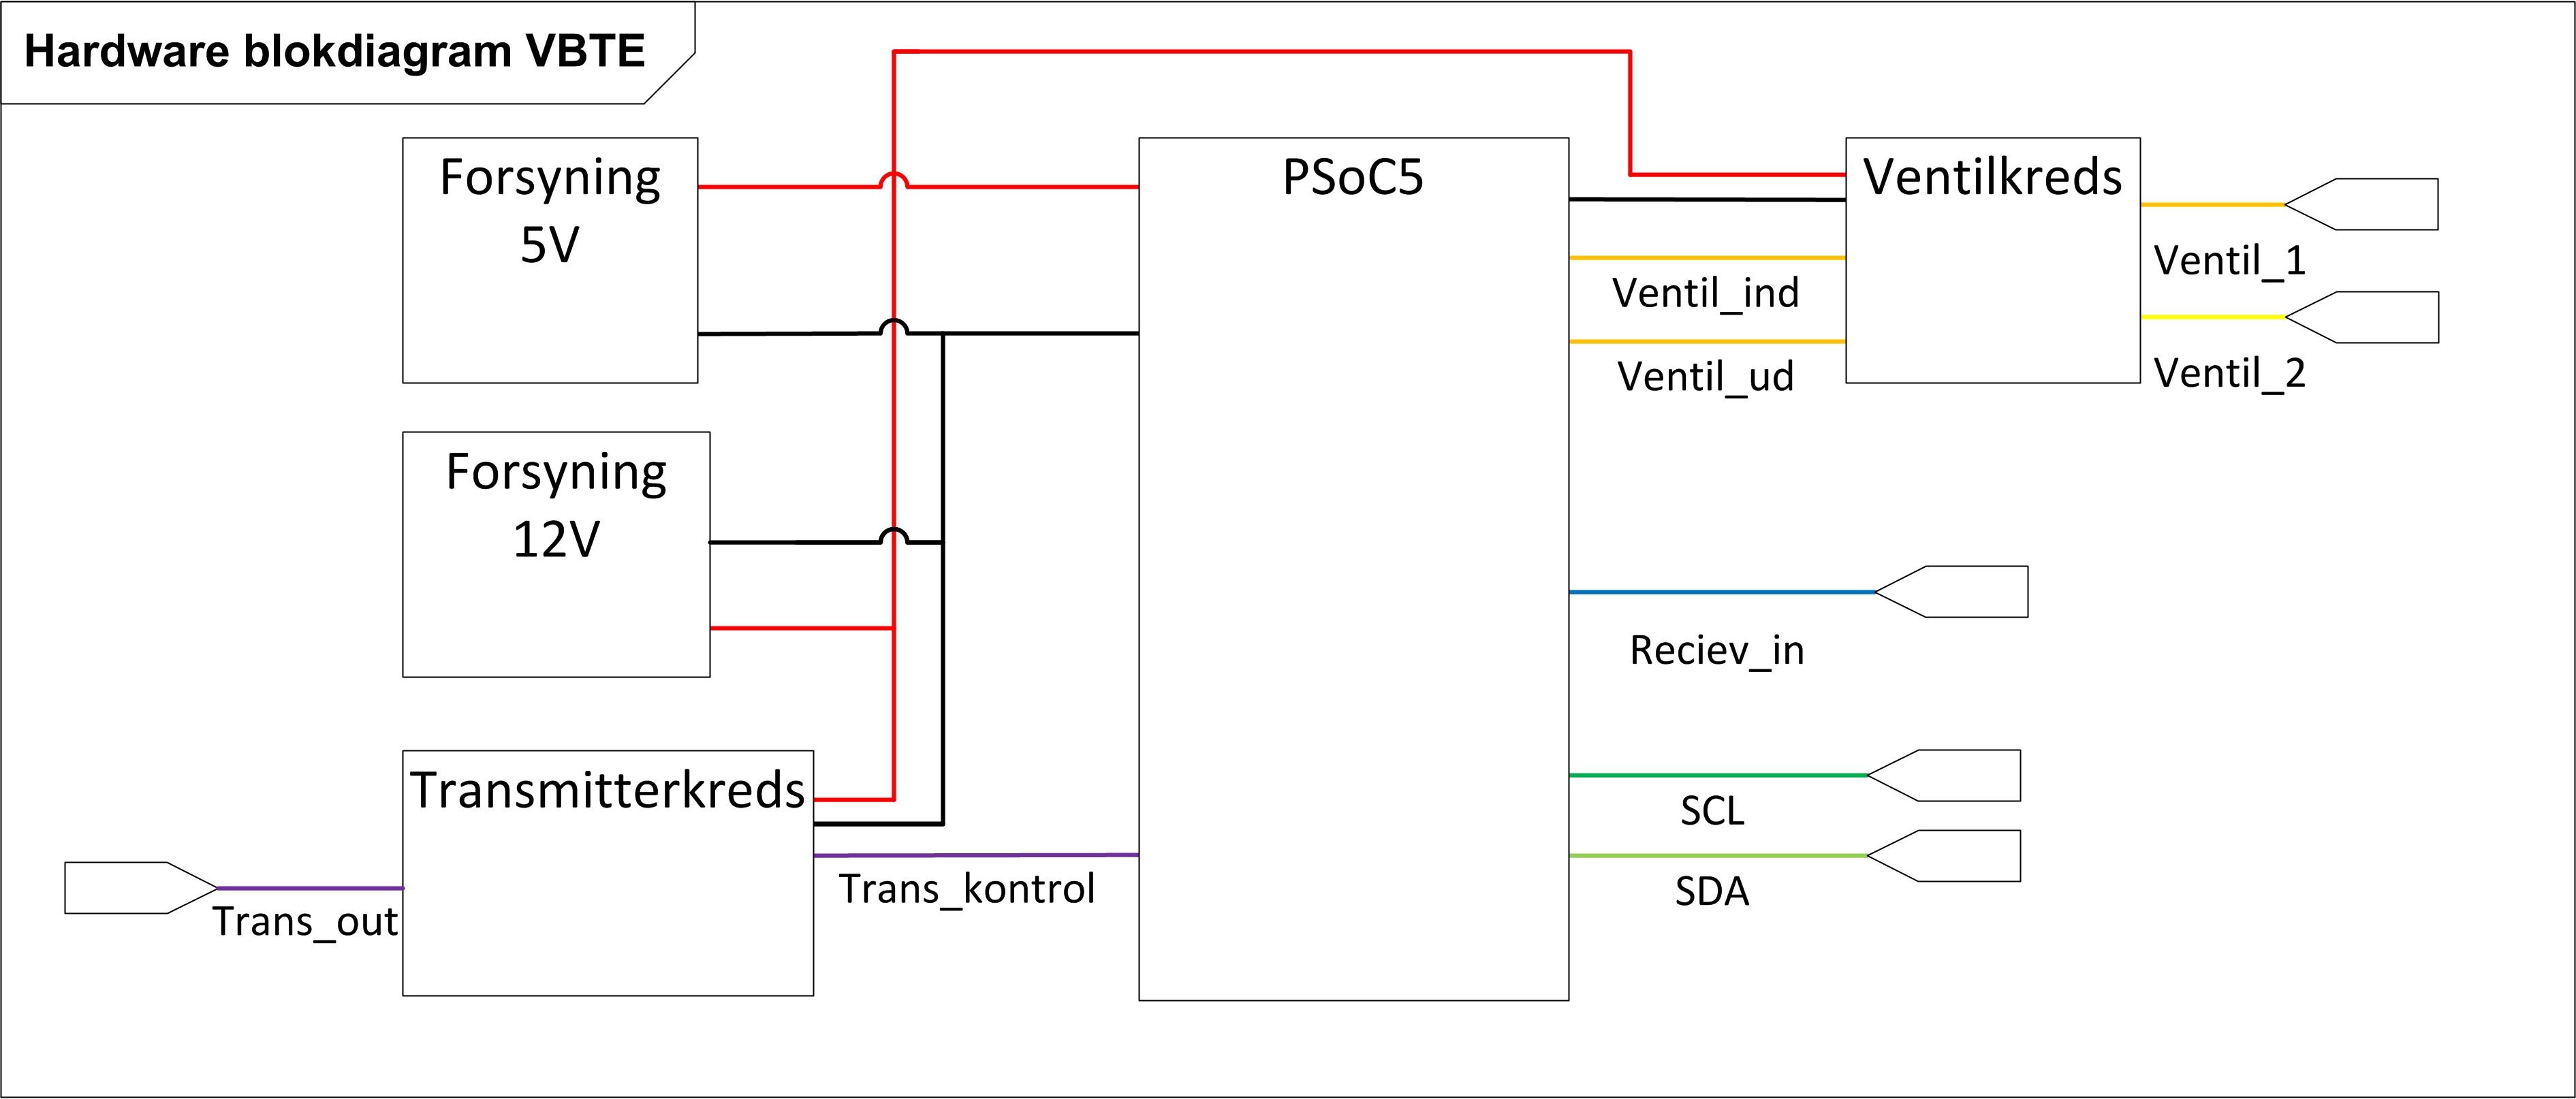
\includegraphics[width = 0.9\textwidth]{billeder/HWVBTE}
\caption{Illustrering af overordnet design af hardware på VBTE.}
\label{fig:HWVBTE}
\end{figure}

\subsubsection{Software}